\documentclass{article}

% Pass 'final' to the neurips_2023 package to remove line numbers if needed
\usepackage[final]{neurips_2023}

\usepackage{graphicx}

\usepackage{enumitem}

% \usepackage{placeins}

\usepackage[utf8]{inputenc} % allow utf-8 input
\usepackage[T1]{fontenc}    % use 8-bit T1 fonts
\usepackage{hyperref}       % hyperlinks
\usepackage{url}            % simple URL typesetting
\usepackage{booktabs}       % professional-quality tables
\usepackage{amsfonts}       % blackboard math symbols
\usepackage{nicefrac}       % compact symbols for 1/2, etc.
\usepackage{microtype}      % microtypography
\usepackage{xcolor}         % colors

\usepackage{hyperref}
\usepackage{cleveref}

\title{Summarization: Learning with Contextual Information in Non-Stationary Environments}

% Paper BibTex
% @inproceedings{anderson2025learning,
%   title={Learning with contextual information in non-stationary environments},
%   author={Anderson, Sean and Hespanha, Joao P},
%   year={2025},
%   organization={7th Annual Learning for Dynamics \& Control Conference (L4DC 2025~…}
% }

\author{
  Summarized by Xiaonan (Nice) Wang \thanks{wangxiaonannice@gmail.com} \\
  % Paper fr last-names (year)
  Summarization\thanks{\textbf{Disclaimer:} This summarization is for research and study purposes. It represents a personal interpretation and may contain inaccuracies. Feedback or corrections via email are highly appreciated.} Generated based on Paper from Anderson and Hespanha. (2025) \\
  Topic: Boltzmann Learning, Non-Stationary Environments, Learning-based Control, Reinforcement Learning\\
}

\begin{document}

\newcommand{\repeatfootnote}[1]{\textsuperscript{\ref{#1}}}

\maketitle

\begin{abstract}
This document summarizes the core contributions and methodology of the paper "Learning with Contextual Information in Non-Stationary Environments, \cite{anderson2025learning}", focusing on its' main ideas and the core blocks.
\end{abstract}

\section{Overview: Core Questions and Answers}
                           
\paragraph{(1) What is the problem?} 
\begin{itemize}
  \item \textbf{Repeated decision-making} with \textbf{contextual (or side) information} in \textbf{non-stationary} environments, where the decision-maker lacks a model (or \textit{priori knowledge}) of the \textit{relationship between actions, contexts, and costs}.
  \begin{itemize}
    \item (\textbf{Boltzmann}) Learning based decision-making.
    \item Non-stationary Environments: Environmental distributions change with time without a stationary model -> preventing \textit{Bayesian optimal} decision based on past data.
    \item 3 elements of modeling:
    \begin{itemize}
      \item \textit{Contextual information (Features)}: measurements (data), side information
      \item \textit{Action}: e.g. Control Signal \& Dynamic (Robotics)
      \item \textit{Cost \& Reward (Optimization Target)}: Costs \& Rewards of Actions (Robotics \& RL)
    \end{itemize}
  \end{itemize}
\end{itemize}

\paragraph{(2) Why need to solve this problem?}
\begin{itemize}
  \item In many \textbf{real-world} domains, \textit{first-principle} models are unavailable and \textbf{learning from data} is necessary.
  \item Non-stationary: Because involving strategic agents who \textbf{observe} and \textbf{react} to past decisions, using standard Bayesian optimal decision-making which relies purely on \textit{stationary past} data is unrealistic.
\end{itemize}

\paragraph{(3) How is it different from prev.?}
\begin{itemize}
  \item Unlike traditional approaches that evaluate average regret over \textit{the whole set of past decisions}, this work introduces a new form of \textbf{exponentially weighted "soft window" regret} (i.e. \textbf{exponentially decaying weights} of the costs).
  \begin{itemize}
    \item By the way, soft windows are \textbf{more computationally efficient} than \textit{fixed windows}.
  \end{itemize}
  \item It also broadens the scope of contextual information by \textbf{extending} finite measurements to the \textbf{continuum} measurement setting (i.e. using the \textit{probability} of measurement's type).
\end{itemize}

\paragraph{(4) Why is it better than prev.? (Advantages)} 
\begin{itemize}
  \item The algorithm provides \textbf{explicit bounds on the regret}, showing that \textbf{regret can be made arbitrarily small}.
  \begin{itemize}
    \item Conceptually, the regret is defined as: $R(T) = \Delta(\pi_{actual}, \pi_{static}^*)$
  \end{itemize}
  \item It is \textbf{computationally much more efficient} and requires significantly \textbf{less memory} than competing \textit{machine learning approaches} (SVM and Neural Network, which must be \textit{continuously retrained on sliding windows of past data} to handle non-stationarity).
\end{itemize}

\paragraph{(5) What is the approach itself?}
\begin{itemize}
  \item Boltzmann Learning
  \begin{itemize}
    \item Calculating an \textbf{"energy"} for each action based on \textbf{past exponentially-discounted costs} associated with the given measurement context;
    \item The agent then \textbf{stochastically} selects actions using a \textbf{Boltzmann distribution} based on these computed energies.
  \end{itemize}
  \item Novelties
  \begin{itemize}
    \item Extension of Contextual Information (Measurements) to \textbf{Continuum} Spaces
    \item \textbf{Exponentially Discounted} Regret (\textbf{"Soft Windows"})
    \item Highly \textbf{Efficient}, \textbf{Lightweight Boltzmann Learning} Architecture
    \item Rigorous Theoretical \textbf{Regret Bounds} (With \textbf{Probability One})
  \end{itemize}
\end{itemize}

\paragraph{(6) What are the applications of it?} 
\begin{itemize}
  \item Numerous real-world domains: clinical trials, portfolio selection, pricing, recommender systems, anomaly detection, cyber security, etc.
  \item Lightweight Learning based Explainable Robotics Control -> Hopefully embedded in real-worl robotics systems.
\end{itemize}

\section{The Structure}

\paragraph{Summarized Block-Diagram} 

The summarized block-diagram of \textit{Exponentially Discounted Regret based Boltzmann Learning} see \cref{fig:boltzmann}\footnote{For efficiency, this diagram was initially hand-drawn on paper and then converted into its current digital version using Nano Banana Pro.}.

\begin{figure}[tb]
  \centering
  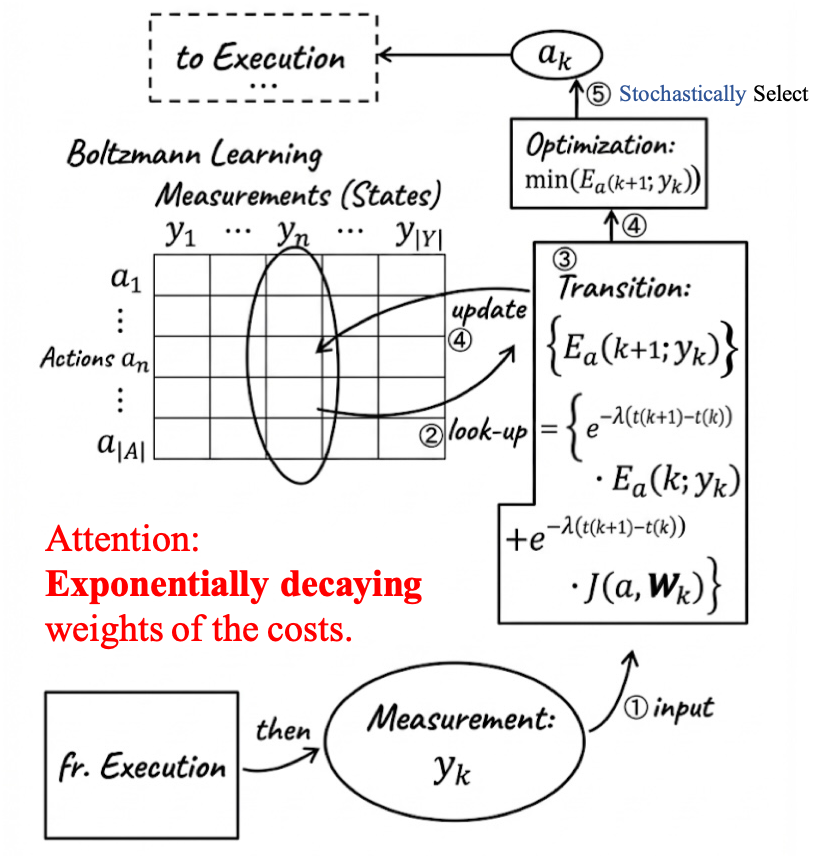
\includegraphics[width=0.95\textwidth]{fig/boltzmann.png}
  \caption{Summarized Block-Diagram of Exponentially Discounted Regret based Boltzmann Learning}
  \label{fig:boltzmann}
\end{figure}

% \paragraph{Original in Paper}

% The original block-diagram see \cref{fig:original}.

% \begin{figure}[tb]
%   \centering
%   
\includegraphics[width=0.95\textwidth]{fig/orig.png}
%   \caption{Original Block-Diagram in Paper}
%   \label{fig:original}
% \end{figure}

\section{Open Questions}

% \begin{enumerate}
%     \item \textbf{Generalizing to Highly Stochastic Environments:}
%     In highly stochastic environments, such as rocky terrains or slippery surfaces, complex maneuvers are often essential for survival. Does forcibly compressing the fractal dimension risk compromising the agent's performance in high-difficulty settings? Furthermore, is there an ``optimal dimension'' that strikes a balance between guaranteed verifiability and environmental adaptability?
%     \item \textbf{Beyond the Model-Free RL:} 
%     Beyond the field of Model-Free RL, does the concept of Fractal Regularization still hold significant value in legged locomotion based on recent popular approaches?
% \end{enumerate}

\bibliographystyle{abbrvnat}
\bibliography{main}

\end{document}
